\documentclass[10pt, article, oneside, margin=1in]{memoir}
\usepackage{hkn}
\usepackage[margin=1in]{geometry}

\begin{document}
	\maketitle
	
	Please find the course notes for CS61A Structure and Interpretation of Computer Programs below, closely following the Fall 2022 asynchronous lecture videos by Professors John Denero and Justin Yokota. A special thank-you to Simon Kuang (simontheflutist@berkeley.edu) for the template.
	
	\tableofcontents*
	\newpage

	\chapter{Functions and Expressions}

\section{Expressions}
\begin{itemize}
	\item Call expression anatomy: <Operator>(<Operands>)
	\item Call expressions evaluate to \emph{values}
	\item Order of evaluation:
	\begin{itemize}
		\item Evaluate operator
		\item Evaluate operands
		\item Apply operator function onto operand values
	\end{itemize}
	\item Primitive expressions
	\begin{itemize}
		\item Number: 2
		\item Name: add
		\item String: 'hello'
	\end{itemize}
\end{itemize}

\section{Environment Diagrams}
\medskip
\begin{figure}[H]
  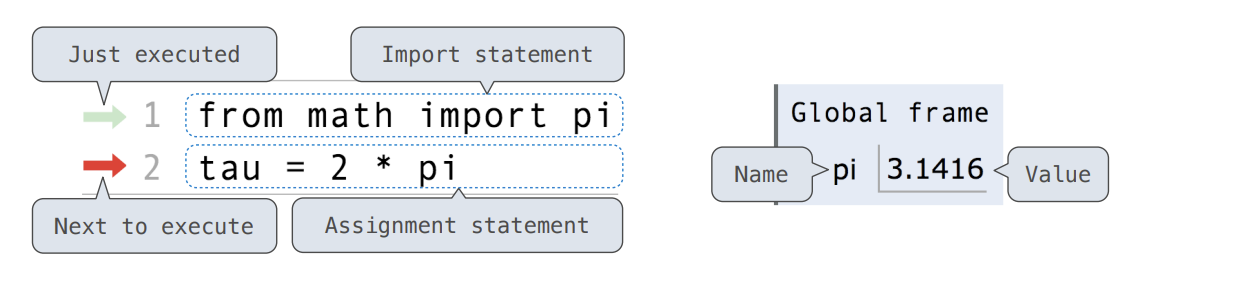
\includegraphics[width=1\linewidth]{figures/environment_diagram.png}
  \caption{Example Environment Diagram}
\end{figure}
\begin{itemize}
	\item Visualization fo the interpreter's process
	\item Left side: statements and expressions
	\begin{itemize}
		\item Arrows indicate evaluation order
	\end{itemize}
	\item Right side: names bounded to values in frames
	\begin{itemize}
		\item Names cannot be repeated in the same frame
		\item An environment in a \emph{sequence of frames}: a frame, its parent frame, and so on
		\item A name evaluates to the value bound to the name in the \emph{earliest frame} of the current environment
		\item Look in the local frame, then in the parent frame, and so on until the global frame
		\item Every expression is evaluated in the context of its environment
	\end{itemize}
	\item Assignment statements: right side is evaluated, and resulting value(s) are binded to the name(s) on the left side
\end{itemize}

\section{Functions}
\begin{itemize}
	\item Function signature anatomy: <name>(<formal parameters>)
	\item Execution order for applying user-defined functions:
	\begin{enumerate}
		\item Create local frame
		\item Bind formal parameters to arguments
		\item Execute the function body in the local frame
	\end{enumerate}
	\item None represents nothing
	\item The return statement completes the evaluation of the call expression
    \item A function that does not explicitly return a value returns None
    \item Pure function: just returns a value
    \item Non-pure function: has side effects
\end{itemize}

\section{Statements}
\begin{itemize}
	\item A statement is \emph{executed by the interpreter to perform an action}
	\medskip
	\begin{figure}[H]
	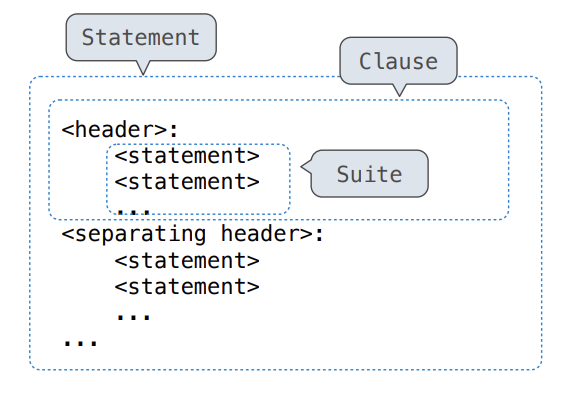
\includegraphics[width=0.5\linewidth]{figures/compound_statement.png}
	\caption{Compound Statement Anatomy}
	\end{figure}
	\item Conditional statement: if clause, followed by elif/else clauses
	\item Execution:
	\begin{enumerate}
		\item Evaluate header expression
		\item If true, execute the suite and skip the remaining clauses
	\end{enumerate}
	\item False values in Python: False, 0, '', None
	\item True values are anything else
	\item While statements (iteration)
	\item Execution:
	\begin{enumerate}
		\item Evaluate header expression
		\item If true, execute the suite and return to step 1
	\end{enumerate}
\end{itemize}
	\chapter{More Functions}

\section{Functions}
\begin{itemize}
    \item Function domain: the set of all inputs that are possible for arguments
    \item Function range: the set of all output values that are possible to return
    \item Function behavior: the relationship between input and output
    \item A function is an abstraction for its effect, behavior, or return value
    \item Functions are a type of value
    \item Higher-order function: a function that takes a function as an argument or returns a function
    \item Higher-order functions can be described with environment diagrams
    \item Self-reference: returning a function using its own name
    \item Parent frame of a function: the frame in which the function was \emph{defined}
\end{itemize}

\section{Lambda Expressions}
\begin{itemize}
    \item Lambda expression: an expression that evaluates to a function
    \item Anatomy: lambda <arguments>: <single expression that evaluates to return value>
    \item Lambda expressions cannot contain statements
    \item "def" vs. "lambda": only def gives the function an intrinsic name in environment diagrams (doesn't affect execution)
    \item Function currying: transforming a multi-argument function into a single-argument, higher-order function
\end{itemize}    

\section{Logical Operators}
\begin{itemize}
    \item Evaluation of <left> and <right>:
    \begin{enumerate}
		\item Evaluate <left>
		\item If the result is False, then the whole expression evaluates to False
		\item Otherwise, the whole expression evaluates to <right>
	\end{enumerate}
    \item Evaluation of <left> or <right>:
    \begin{enumerate}
		\item Evaluate <left>
		\item If the result is True, then the whole expression evaluates to Talse
		\item Otherwise, the whole expression evaluates to <right>
	\end{enumerate}
\end{itemize}

\section{Errors}
\begin{itemize}
    \item Syntax errors: detected by Python interpreter before execution
    \item Runtime errors: detected by Python interpreter during execution
    \item Logic \& behavior errors: Not detected by the Python interpreter
\end{itemize}

\section{Recursion}
\begin{itemize}
    \item Recursive function: a function that calls itself, directly or indirectly
    \item Usage: solving problems that \emph{have smaller instances of the same problem}
    \item Anatomy:
    \begin{itemize}
        \item "def" statement header
        \item Conditional statements that check for \emph{base cases}
        \item Base cases are evaluated \emph{without recursive calls}
        \item Recursive cases (all other cases) are evaluated \emph{with recursive calls}
    \end{itemize}
    \item The recursive leap of faith: assumption that the smaller case is solved correctly to solve the current case
    \item Iteration is a special case of recursion
    \item Tree recusion: a recursive function makes more than one recursive call
\end{itemize}
	\chapter{Sequences}

\section{Lists and Containers}
\begin{itemize}
    \item List: a compound value (sequence of values)
    \item A method of combining data values satisfies the \emph{closure property} if the result of the combination can itself be combined using the same method
    \item i.e. Lists can contain lists as elements
    \medskip
	\begin{figure}[H]
	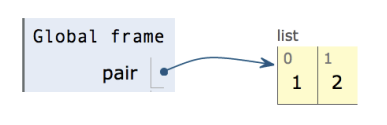
\includegraphics[width=0.5\linewidth]{figures/env_diagram_list.png}
	\caption{List Format in Environment Diagrams}
	\end{figure}
\end{itemize}

\section{For Statements}
\begin{itemize}
    \item Anatomy: for <name> in <expression>:
    \item Execution:
    \begin{enumerate}
        \item evaluate <expression>, which must yield an iterable value (sequence)
        \item For each element in that sequence in order: 
        \begin{enumerate}
            \item Bind <name> to that element in the current frame
            \item Execute the suite
        \end{enumerate}
    \end{enumerate}
\end{itemize}

\section{Ranges}
\begin{itemize}
    \item Range: a sequence of consecutive integers
    \item Starting value (inclusive) to enging value (exclusive)
    \item Length: ending value - starting value
\end{itemize}

\section{List Comprehensions}
\begin{itemize}
    \item Combined expression that evaluates to a list
    \item Anatomy: [<map exp> for <name> in <iter exp> if <filter exp>]
    \item Anatomy without filter: [<map exp> for <name> in <iter exp>]
    \item For each element in <iter exp> if <filter exp> is True, then add <map exp>
\end{itemize}

\section{Slicing}
\begin{itemize}
    \item Slicing a list creates new values, does not reference original list values
    \item Anatomy: <new list name> = <list name>[<start index>:<end index>]
    \item If no explicit start or end index, the beginning or end of the list is used
    \item Start index is inclusive, end index is exclusive
\end{itemize}

\section{Aggregation}
\begin{itemize}
    \item Built-in functions:
    \item sum(iterable[, start]) -> value
    \item Returns the sum of an iterable + start (default start value is 0)
    \item max(iterable[, key=func]) -> value
    \item Returns the largest item in the iterable, based on key function (default is no function)
    \item all(iterable) -> value
    \item Returns True if all values in the iterable are True (including empty iterable), False otherwise
\end{itemize}

\section{Strings}
\begin{itemize}
    \item String literabls are surrounded with single or double quotes
    \item A backslash "\textbackslash" escapes the next character
    \item Line feed character "\textbackslash n" represents a new line
\end{itemize}

\section{Dictionaries}
\begin{itemize}
    \item Dictionary: a collection of key-value pairs
    \item Keys must be unique within the same dictionary
    \item Keys cannot be a list or dictionary
    \item Dictionary comprehension: \{<key exp>: <value exp> for <name> in <iter exp> if <filter exp>\}
\end{itemize}
	\chapter{Abstraction}

\section{Data Abstraction}
\begin{itemize}
    \item Data abstrction: a methodology by which functions enforce an abstraction barrier between \emph{representaion} and \emph{use}
    \item Identify a basic set of operations in which all manipulations of a data type can be expressed, then use only those operations for manipulating that data
    \item Abstraction barriers separate stages of an implementation into levels of abstraction
    \item Example - rational numbers:
    \medskip
	\begin{figure}[H]
	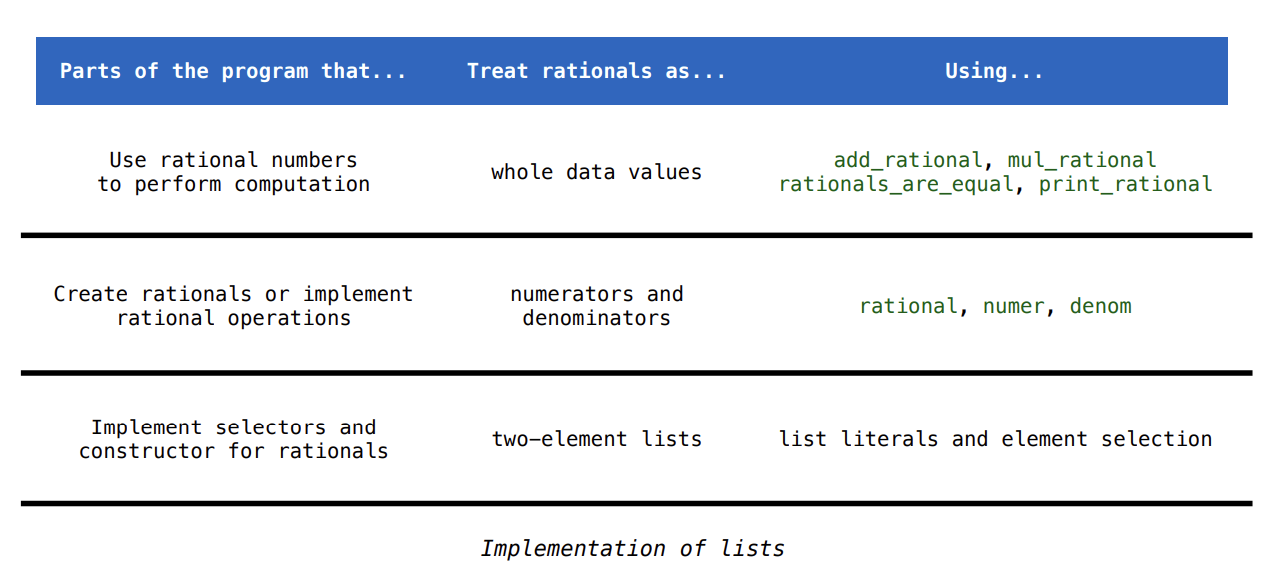
\includegraphics[width=1\linewidth]{figures/data_abstraction.png}
	\caption{List Format in Environment Diagrams}
	\end{figure}
\end{itemize}
	\chapter{Mutability}

\section{Objects}
\begin{itemize}
    \item Objects represent \emph{information} and consist of attributes - \emph{data} and \emph{behavior}
    \item A type of onject is called a \emph{class}
    \item Object-oriented programming: a methodology for organizing larger programs by:
    \begin{itemize}
        \item Using data abstraction
        \item Bundling together information and related behavior (objects)
    \end{itemize}
    \item Functions do one thing, objects do \emph{many related things}
    \item Mutability: the ability for an object to change
\end{itemize}

\section{Tuples}
\begin{itemize}
    \item Tuple: an immutable sequence
    \item An immutable sequence can still be changed if it \emph{contains} a mutable value as an element
\end{itemize}

\section{Identity Operators}
\begin{itemize}
    \item Identity: <exp0> is <exp1>
    \item True if both <exp0> and <exp1> evaluate to the \emph{same object}
    \item Equality: <exp0> == <exp1>
    \item True if both <exp0> and <exp1> evaluate to \emph{equal values}
\end{itemize}

\section{Files, Strings, and Lists}
\begin{itemize}
    \item .strip() : returns a string without whitespace on the ends
    \item .split() : returns a list of strings that were separated by whitespace
    \item .replace(a, b) : returns a string with all instances of string a replaced by string b
\end{itemize}
	\chapter{Iterators and Generators}

\section{Iterators}
\begin{itemize}
    \item Any container can provide an iterator that provides elements in Order
    \item iter(iterable) : returns an iterator
    \item next(iterator) : returns the next element in an iterator
    \item For dictionaries, the order of items (key-value pairs) is the order in which they were added
    \item Iterators make few assumptions about the data, so others are more likely to be able to use your code on their data
    \item Iterators keep track of position within the sequence, ensuring each element is only processed once
\end{itemize}

\section{Built-In Functions for Iteration}
\begin{itemize}
    \item map(func, iterable) : iterate over x in iterable using func(x)
    \item filter(func, iterable) : iterate over x in iterable if func(x)
    \item zip(iter1, iter2): iterate over co-indexed (x, y) pairs, 
    \begin{itemize}
        \item Skips extras if iterables are different length
        \item Can take more than two lists as arguments
    \end{itemize}
    \item reversed(sequence) : iterate over x in a sequence in reverse order
    \item Functions to view the contents of an iterator:
    \item list(iterable) : return a list containing all x in iterable
    \item tuple(iterable) : return a tuple containing all x in iterable
    \item sorted(iterable) : return a sorted list containing all x in iterable
\end{itemize}

\section{Generators}
\begin{itemize}
    \item Generator: a function that \emph{yields} values instead of returning them
    \item A generator can yield multiple times
    \item A generator is an iterator that is created by calling a \emph{generator function}
    \item "yield from" statement yields all values from an iterator/iterable
\end{itemize}
	\chapter{Objects}

\section{Classes}
\begin{minted}[tabsize=4]{Python}
    class <name>:
        <suite>
\end{minted}
\begin{itemize}
    \item Class: a type/category of objects
    \item Objects are created by calling Classes
    \item Classes are objects as well
    \item Every object that is an instance of a user-defined class has a unique identity
    \item "is" and "is not" test if two expressions evaluate to the same object
    \item Binding an object to a new name using assignment does not create a new object
    \item Methods are functions definined in the suite of a class statement
    \item Defining methods:
\end{itemize}
\begin{minted}[tabsize=4]{Python}
    class <class name>:
        def <method name>(self, <formal parameters>):
            <suite>
\end{minted}
\begin{itemize}
    \item Dot expressions: <exp>.<name>
    \begin{itemize}
        \item <exp> must evaluate to an object
        \item If <name> is a method, then "self" parameter is automatically supplied
        \item Evaluation order:
        \begin{enumerate}
            \item Evaluate <exp>
            \item <name> is looked up in the instance attributes of that object
            \item If not found, <name> is looked up in the class
            \item If the value is a function, a bound method is returned. If not, the value is returned
        \end{enumerate}
    \end{itemize}
    \item Looking up an attribute using a string: getattr(<object expression>, "<name>")
    \item Instance attributes are attributes of a specific object instance
    \item Class attributes are shared across all instances of a class
    \item Assignment using dot expressions: <exp1>.<name> = <exp2>
    \begin{itemize}
        \item The value of <exp2> is binded to the attribute <name> found in the evaluated <exp1> object
    \end{itemize}
\end{itemize}

\section{Inheritance}
\begin{itemize}
    \item Inheritance: a technique for relating classes together
    \item Often used for specialization
\end{itemize}
\begin{minted}[tabsize=4]{Python}
    class <class name>(<base class>):
        <suite>
\end{minted}
\begin{itemize}
    \item Subclass inherits attributes of its base class
    \item Certain inherited attributes may be overridden
    \item Base class attributes are not copied into subclasses
    \item Inheritance is best for representing \emph{is-a relationships}
    \item Composition is best for representing \emph{has-a relationships}
    \item A class may inherit from multiple base classes in Python
\end{itemize}

\section{Representation}
\begin{itemize}
    \item All objects have two forms of string representations
    \item "str" is legible to humans (same value as what is printed with "print" function)
    \item "repr" is legible to the Python interpreter
    \item For most object types, eval(repr(object)) == object
    \item F-Strings for string interpolation
    \begin{itemize}
        \item String interpolation: evaluating a string literal that contains expressions
        \item Equivalent examples:
        \item String concatenation: 'pi starts with ' + str(pi) + '...'
        \item String interpolation: f'pi starts with \{pi\}...'
        \item Equivalent output: 'pi starts with 3.141592653589793...'
    \end{itemize}
\end{itemize}

\section{Polymorphic Functions}
\begin{itemize}
    \item Polymorphic function: a function that applies to many different forms of data
    \item Examples: "str" and "repr"
\end{itemize}

\section{Interfaces}
\begin{itemize}
    \item Interface: a set of shared messages, along with a specification of what they management
    \item Example: classes that implement \_\_repr\_\_ and \_\_str\_\_ methods that return string representations implement an interface for producing string representations
\end{itemize}

\section{Special Method Names in Python}
\begin{itemize}
    \item \_\_init\_\_ : method invoked automatically when an object is construction
    \item \_\_repr\_\_ : method invoked to display an object as a Python expression
    \item \_\_add\_\_ : method invoked to add one object to another
    \item \_\_bool\_\_ : method invoked to convert an object to True or False
    \item \_\_float\_\_ : method invoked to convert an object to a float
\end{itemize}

\section{Generic Functions}
\begin{itemize}
    \item A polymorphic function may take arguments that vary in types
    \item Type dispatching: inspect the type of an argument to select behavior
    \item Type coercion: convert one value to math the type of another
\end{itemize}
	\chapter{Composition}

\section{Linked Lists}
\begin{itemize}
    \item Linked list structure: a linked list is either empty or a first value and the rest of the linked list
    \item Linked lists are mutable
    \medskip
	\begin{figure}[H]
	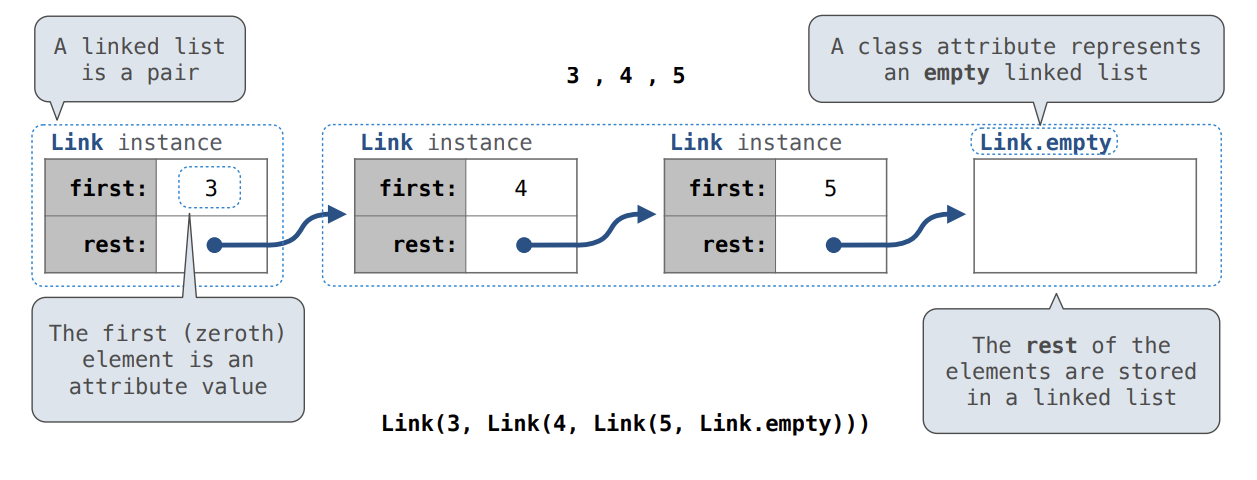
\includegraphics[width=1\linewidth]{figures/linked_list_example.png}
	\caption{Linked List Example}
	\end{figure}
\end{itemize}
\begin{minted}[tabsize=4]{Python}
    class Link:
        empty = () # some zero-length sequence
        def __init__(self, first, rest=empty):
            assert rest is Link.empty or isinstance(rest, Link) # verify rest is a linked list
            self.first = first
            self.rest = rest
\end{minted}

\section{Trees}
\begin{itemize}
    \item Recursive description of trees
    \begin{itemize}
        \item A tree has a root label and a list of branches
        \item Each branch is a tree
        \item A tree with zero branches is called a leaf
        \item A tree starts at the root
    \end{itemize}
    \item Relative description of trees
    \begin{itemize}
        \item Each location in a tree is called a node
        \item Each node has a label that can be any value
        \item One node can be the parent/child of another
        \item The top node is the root node
    \end{itemize}
    \item Tree processing often uses recursion, with the leaf as a base case
    \item Example tree implementation:
\end{itemize}
\begin{minted}[tabsize=4]{Python}
    class Tree:
        def __init__(self, label, branches=[]):
            self.label = label
            for branch in branches:
                assert isinstance(branch, Tree)
            self.branches = list(branches)
            for branch in branches:
        def tree(label, branches=[]):
            for branch in branches:
                assert is_tree(branch)
            return [label] + list(branches)
        def label(tree):
            return tree[0]
        def branches(tree):
            return tree[1:]
\end{minted}
\begin{itemize}
    \item Pruning: removing subtrees from a tree
    \item Pruning can be used before recursive processing to speed up computation
\end{itemize}

\section{Modular Design}
\begin{itemize}
    \item A design principle: isolate different parts of a program that address different concerns
    \item Each modular component can be developed and tested independently
    \item Example:
    \medskip
	\begin{figure}[H]
	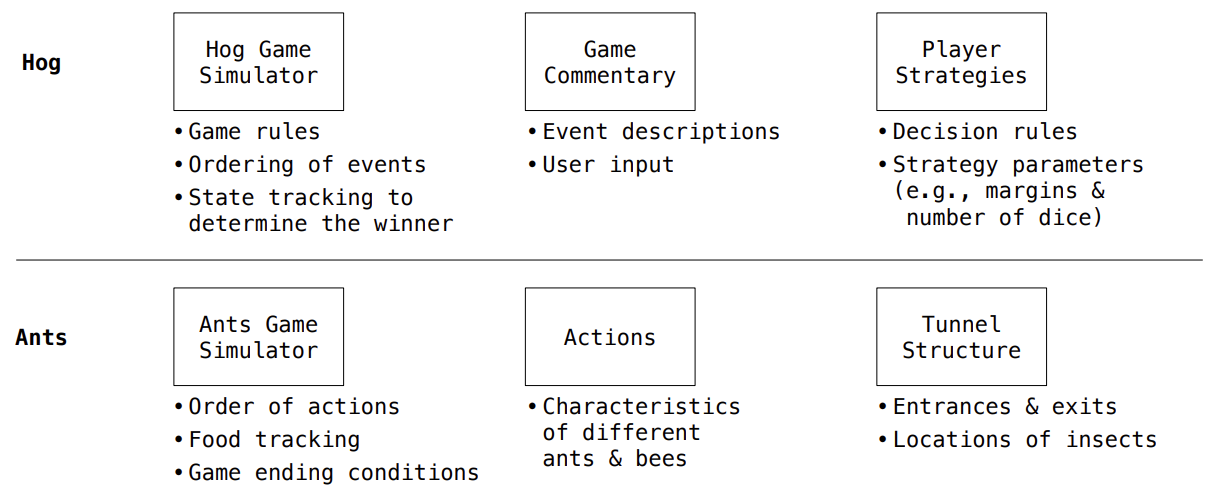
\includegraphics[width=1\linewidth]{figures/modular_design_example.png}
	\caption{Modular Design Example}
	\end{figure}
\end{itemize}
	\chapter{Efficiency}

\section{Memoization}
\begin{itemize}
    \item Memoization: "remembering" the results that have been computed before
    \item Example - fibonacci numbers:
    \item Store the $n^{th}$ fibonacci number in a cache so that its value can be used to compute larger fibonacci numbers later
\end{itemize}

\section{Exponentiation}
\begin{itemize}
    \item Taking advantage of repeated multiplication
    \item One more multiplication allows the problem size to be doubled
    \item Example:
\end{itemize}
\begin{minted}[tabsize=4]{Python}
    # doubling imput doubles the time
    def exp(b, n):
        if n == 0:
            return 1
        else:
            return b * exp(b, n-1)

    # doubling the input increases the time by one step
    def exp_fast(b, n):
        if n == 0:
            return 1
        elif n % 2 == 0:
            return square(exp_fast(b, n//2))
        else:
            return b * exp_fast(b, n-1)

    def square(x):
        return x * x
\end{minted}

\section{Orders of Growth}
\begin{description}
    \item [Constant growth - $\Theta(1), O(1)$:] increasing n doesn't increase time
    \item [Logarithmic growth - $\Theta(\log n), O(\log n)$:] doubling n increases time by a constant
    \item [Linear growth - $\Theta(n), O(n)$:] incrementing n increases time by a constant
    \item [Quadratic growth - $\Theta(n^2), O(n^2)$:] incrementing n increases time by n * constant
    \begin{itemize}
        \item Example: functions that process all \emph{pairs} of values in a sequence
    \end{itemize}
    \item [Exponential growth - $\Theta(b^n), O(b^n)$:] incrementing n multiplies time by a constant
    \begin{itemize}
        \item Example: tree-recursive functions (fibonacci without memoization)
    \end{itemize}
\end{description}

\section{Space}
\begin{itemize}
    \item Active environments: 
    \item Environments for any function calls currently being evaluated
    \item Parent environments of functions named in active environments
\end{itemize}
	\chapter{Data Examples}

\section{Lists in Lists in Environment Diagrams}
\medskip
\begin{figure}[H]
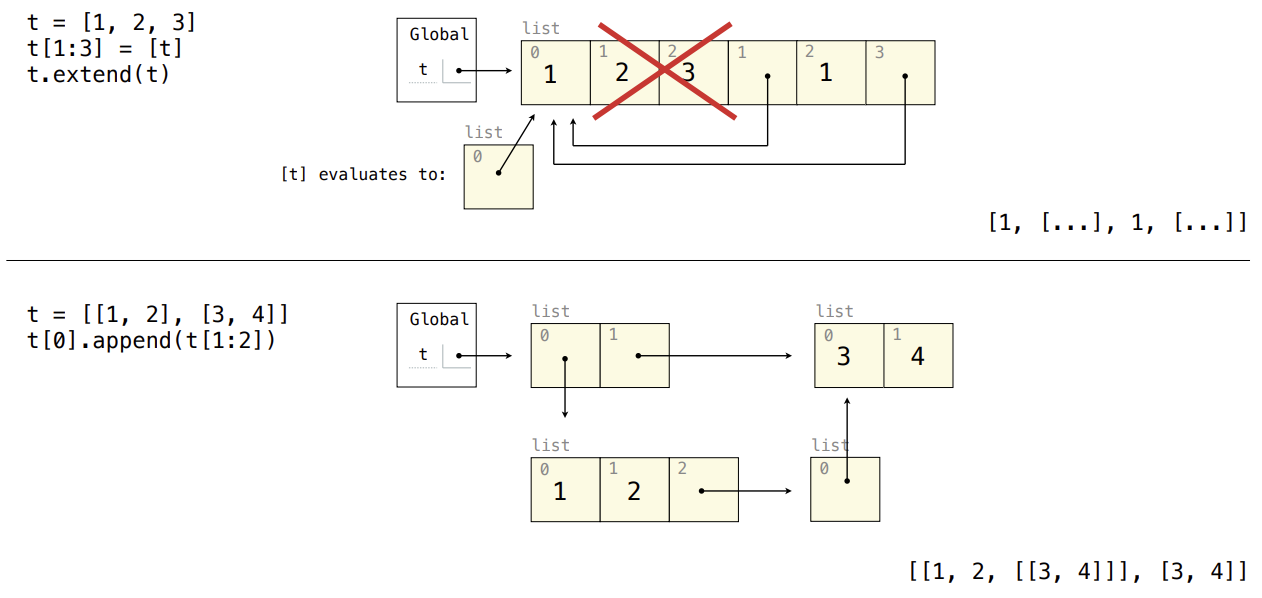
\includegraphics[width=1\linewidth]{figures/lists_in_lists_env_diagram.png}
\caption{Example of Lists within Lists in an Environment Diagram}
\end{figure}

\section{Objects}
	\chapter{Scheme}

\section{Scheme}
\begin{itemize}
    \item Scheme is a dialect of Lisp
    \item Scheme programs consist of expressions:
    \begin{itemize}
        \item Primitive expressions: 2, 3.3, true, +, quotient
        \item Combinations: (quotient 10 2), (not true)
    \end{itemize}
    \item Call expressions incude an operator and 0 or more operands in parentheses
    \item Special forms: combinations that are not call expressions
    \item Examples: \textbf{if}, \textbf{and}, \textbf{or}, binding symbols, defining procedures, \textbf{cond}, \textbf{begin}
    \begin{minted}[tabsize=4]{Scheme}
    (if <predicate> <consequent> <alternative>)

    (and <exp1> ... <expn>)

    (or <exp1> ... <expn>)

    (define <symbol> <expression>)

    (define (<symbol> <formal parameters>) <body>)

    (cond (<predicate 1> <consequent 1>)
          (<predicate 2> (begin <consequent 2a> ... <consequent 2m>))
          ...
          (else <consequent n>))
    \end{minted}
    \item Lambda expressions: 
    \begin{minted}[tabsize=4]{Scheme}
    (lambda (<formal parameters>) <body>)
    \end{minted}
    \item Let expression: binds symbols to values just for one expression
    \begin{minted}[tabsize=4]{Scheme}
    (let <symbol> <expression>)
    \end{minted}
\end{itemize}

\section{Scheme Lists}
\begin{itemize}
    \item Scheme lists are similar to Python linked-lists
    \begin{description}
        \item [cons:] two-argument procedure that creates a linked list
        \item [car:] procedure that returns the first element of a list
        \item [cdr:] procedure that returns the rest of a list
        \item [nil:] the empty list
    \end{description}
    \item Example list:
\end{itemize}
\begin{minted}[tabsize=4]{Scheme}
    > (cons 1 (cons 2 (cons 3 (cons 4 nil))))
    (1 2 3 4)
    > (define x (cons 1 (cons 2 nil)))
    > x
    (1 2)
    > (car x)
    1
    > (cdr x)
    (2)
\end{minted}

\section{Symbolic Programming}
\begin{itemize}
    \item Symbols normally refer to values, single quote is used to refer to symbols directly
\end{itemize}
\begin{minted}[tabsize=4]{Scheme}
    > (define a 1)
    > (define b 2)
    > (list 'a b)
    (a 2)

    > '(a b c)
    (a b c)
    > (car '(a b c))
    a
    > (cdr '(a b c))
    (b c)
\end{minted}

\section{Built-in List Processing Procedures}
\begin{description}
    \item [(append s t):] list the elements of s and t (can be called on more than two lists)
    \item [(map f s):] call a procedure f on each element of a list s and list results
    \item [(filter f s):] call a procedure f on each element of a list s and list the elements for which true is the result
    \item [(apply f s):] call a procedure f using elements of list s as its arguments
\end{description}


	\chapter{Exceptions}

\section{Raise}
\begin{itemize}
    \item Raise statements raise an exception in Python
    \begin{minted}[tabsize=4]{Python}
    raise <expression>
    \end{minted}
    \item <expression must evaluate to a subclass or instance of BaseException
    \begin{itemize}
        \item \textbf{TypeError:} incorrect type of argument was passed into a function
        \item \textbf{NameError:} a name wasn't found
        \item \textbf{KeyError:} a key wasn't found in a Dictionary
        \item \textbf{RecursionError:} too many recursive calls
    \end{itemize}
\end{itemize}

\section{Try}
\begin{itemize}
    \item Try statements handle Exceptions
    \begin{minted}[tabsize=4]{Python}
    try:
        <try suite>
    except <exception class> as <name>:
        <except suite>
    ...
    \end{minted}
    \item Execution order:
    \begin{enumerate}
        \item <try suite> is executed first
        \item If, in the try suite, an exception is raised that is not handled otherwise and if the class exception inherits from <exception class>, then
        \item <except suite> is executed, with <name> bound to the exception
    \end{enumerate}
\end{itemize}
	\chapter{Programming Languages}

\section{Programming Languages}
\begin{description}
    \item [Machine languages:] interpreted by the hardware itself
    \item [High-level languages:] interpreted by another program or compiled into another language
    \begin{itemize}
        \item Abstracts away system details
        \item Creates independence from hardware and operating system
    \end{itemize}
    \item [Syntax:] legal statements and expressions in the language
    \item [Semantics:] execution/evaluation rules for those statements and expressions
\end{description}

\section{Parsing}
\begin{itemize}
    \item Parsing: turning text into an expression
    \item Syntactic analysis: identifying the hierarchical structure of an expression
    \item Evaluation: the computation of the value of an expression
\end{itemize}

\section{Interpreters}
\begin{itemize}
    \item Programs specify the logic of a computational device
    \item An interpreter is a \emph{general computing machine}
\end{itemize}
\medskip
\begin{figure}[H]
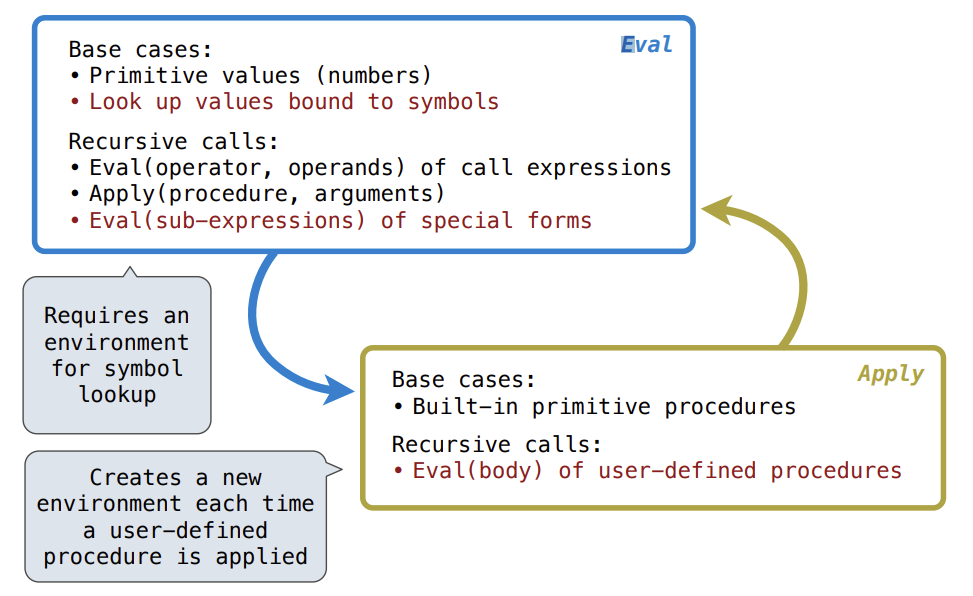
\includegraphics[width=0.8\linewidth]{figures/structure_of_an_interpreter.png}
\caption{Interpreter Structure}
\end{figure}
	\chapter{Tail Recursion}

\section{Dynamic Scope}
\begin{description}
    \item [Lexical scope:] the parent of a frame is the environment in which a procedure was \emph{defined}
    \begin{minted}[tabsize=4]{Scheme}
    (define <symbol> (lambda <formal parameters> <body>))
    \end{minted}
    \item [Dynamic scope:] the parent of a frame is the environment in which a procedure was \emph{called}
    \begin{minted}[tabsize=4]{Scheme}
    (define <symbol> (mu <formal parameters> <body>))
    \end{minted}
\end{description}

\section{Tail Recursion}
\begin{itemize}
    \item Referential transparency: the value of an expression does not change when we substitute one of its subexpressions with the value of that subexpression
    \item Tail recursion eliminates the "middleman" frames to save space
    \item Tail call: a call expression in a tail context
    \begin{itemize}
        \item The last sub-expression in a \textbf{lambda} expression's body
        \item Sub-expressions <consequent> and <alternative> in an \textbf{if} expression that is in a tail context
        \item All non-predicate sub-expressions in a tail context \textbf{cond}
        \item The last sub-expression in a tail context \textbf{and, or, begin,} or \textbf{let}
    \end{itemize}
\end{itemize}

\section{Macros}
\begin{itemize}
    \item Macro: an operation performed on the source code of a program before evaluation
    \item Scheme example:
    \begin{minted}[tabsize=4]{Scheme}
        > (define-macro (twice expr) (list 'begin expr expr))
        > (twice (print 2))
        2
        2
    \end{minted}
\end{itemize}
	\chapter{SQL}

\section{Databases}
\begin{itemize}
    \item Table: a collection of rows that have a value for each column
    \item SQL is a \emph{declarative} programming languages
    \begin{itemize}
        \item \textbf{Declarative language (SQL, Prolog):} a program is a description of the desired result, and the program figures out how to generate the result
        \item \textbf{Imperative language (Python, Scheme):} a program is a description of computational processes that the interpreter carries out
    \end{itemize}
\end{itemize}

\section{SQL}
\begin{itemize}
    \item A \textbf{select} statement creates a new table, either from scratch bor by projecting a table
    \begin{itemize}
        \item Always includes a comma-separated list of column descriptions
    \end{itemize}
    \begin{minted}[tabsize=4]{SQL}
    select [expression] as [name], [expression] as [name]; ...
    select [columns] from [table] where [condition] order by [order];
    \end{minted}
    \item A \textbf{create table} statement gives a global name to a table
    \begin{minted}[tabsize=4]{SQL}
    create table [name] as [select statement];
    \end{minted}
    \item Two or more tables can be joined together
    \begin{minted}[tabsize=4]{SQL}
    select parent from parents, dogs where child = name and fur = "curly"
    \end{minted}
\end{itemize}

\section{Aliases and Dot Expressions}
\begin{itemize}
    \item Aliases and dot expressions clear up ambiguity with column names
    \item Example of using aliases and dot expressions when joining a table with itself:
    \begin{minted}[tabsize=4]{SQL}
    select a.child as first, b.child as second 
        from parents as a, parents as b 
        where a.parent = b.parent and a.child < b.child;
    \end{minted}
    \item Other statements: \textbf{analyze, delete, explain, insert, replace, update,} etc.
    \item Expressions can contain function calls and arithmetic Operators
    \item String values can be combined to form longer strings
    \begin{minted}[tabsize=4]{SQL}
    > select "hello," || " world";
    hello, world
    \end{minted}
\end{itemize}

\section{Aggregate Functions}
\begin{itemize}
    \item An aggregate function in the [columns] clause computes a value from a group of rows
    \begin{minted}[tabsize=4]{SQL}
    select [columns] from [table] where [condition] order by [order];
    \end{minted}
    \item Aggregate functions: \textbf{max, min, avg}
\end{itemize}

\section{Grouping Rows}
\begin{itemize}
    \item Rows in a table can be grouped, then aggregation can be performed on each group
    \item Number of groups is the number of unique values of an expression
    \item A \textbf{having} clause filters the set of groups that are aggregated
    \begin{minted}[tabsize=4]{SQL}
    select [columns] from [table] group by [expression] having [filter expression]
    \end{minted}
\end{itemize}
	\include{lecture16}
	\include{lecture17}
	\include{lecture18}
	\include{lecture19}
	\include{lecture20}
	\include{lecture21}
	\include{lecture22}
	\include{lecture23}
	\include{lecture24}
	\include{lecture25}
	\include{lecture26}
\end{document}